% Fundamental packages
\documentclass[11pt,a4paper,twoside]{book}
\usepackage[utf8]{inputenc}
\usepackage[american]{babel}
\usepackage{amsmath}
\usepackage{amsfonts}
\usepackage{amssymb}
\usepackage{graphicx}

% margins and general lay-out
%\usepackage[inner=3cm,outer=2cm,top=2.5cm,bottom=2.5cm]{geometry}
\usepackage[inner=2.5cm,outer=2.5cm,top=2.5cm,bottom=2.5cm]{geometry}
\pagestyle{plain}

% fonts (Helvetica) and typographical stuff 

\usepackage[T1]{fontenc}
\usepackage{lmodern} 
\usepackage{textcomp} 
\usepackage{pifont}
\usepackage{csquotes}
\usepackage{bm}

% Setting the font should be done after loading the typographic packages which tend to 
% set a new default font. The microtype package should however be loaded after the font ...
% using san serif helvetica clone
\usepackage{helvet}
\renewcommand{\familydefault}{\sfdefault}
% phv is another posibility.
% \renewcommand\rmdefault{phv}
\usepackage{microtype}

% additional packages
\usepackage{booktabs}
\usepackage{pdfpages}
\usepackage{hyperref}
\usepackage{float}
\usepackage{todonotes}
\usepackage{caption}
\usepackage{subcaption}

% package to manage citations
\usepackage[backend=bibtex,style=authoryear-comp,sorting=nyt,isbn=false,url=false]{biblatex}
\addbibresource{Bibliography/Bibliography.bib}

% Kill the auto-indent
\setlength\parindent{0pt}

% test package
\usepackage{lipsum}

% Packages for list of symbols and list of abbreviations
%\usepackage[nonumberlist,acronym,toc,nomain]{glossaries}
%\makeglossaries
%\input{Glossaries/Abbreviations}

% new definitions
\newcommand{\expit}{\text{expit}} 
\DeclareMathOperator*{\argmax}{arg\,max}

\DeclareMathOperator*{\argmin}{arg\,min}


% start of the document
\begin{document}

% include cover page + copyright statement + no pagenumbers
\pagenumbering{gobble}
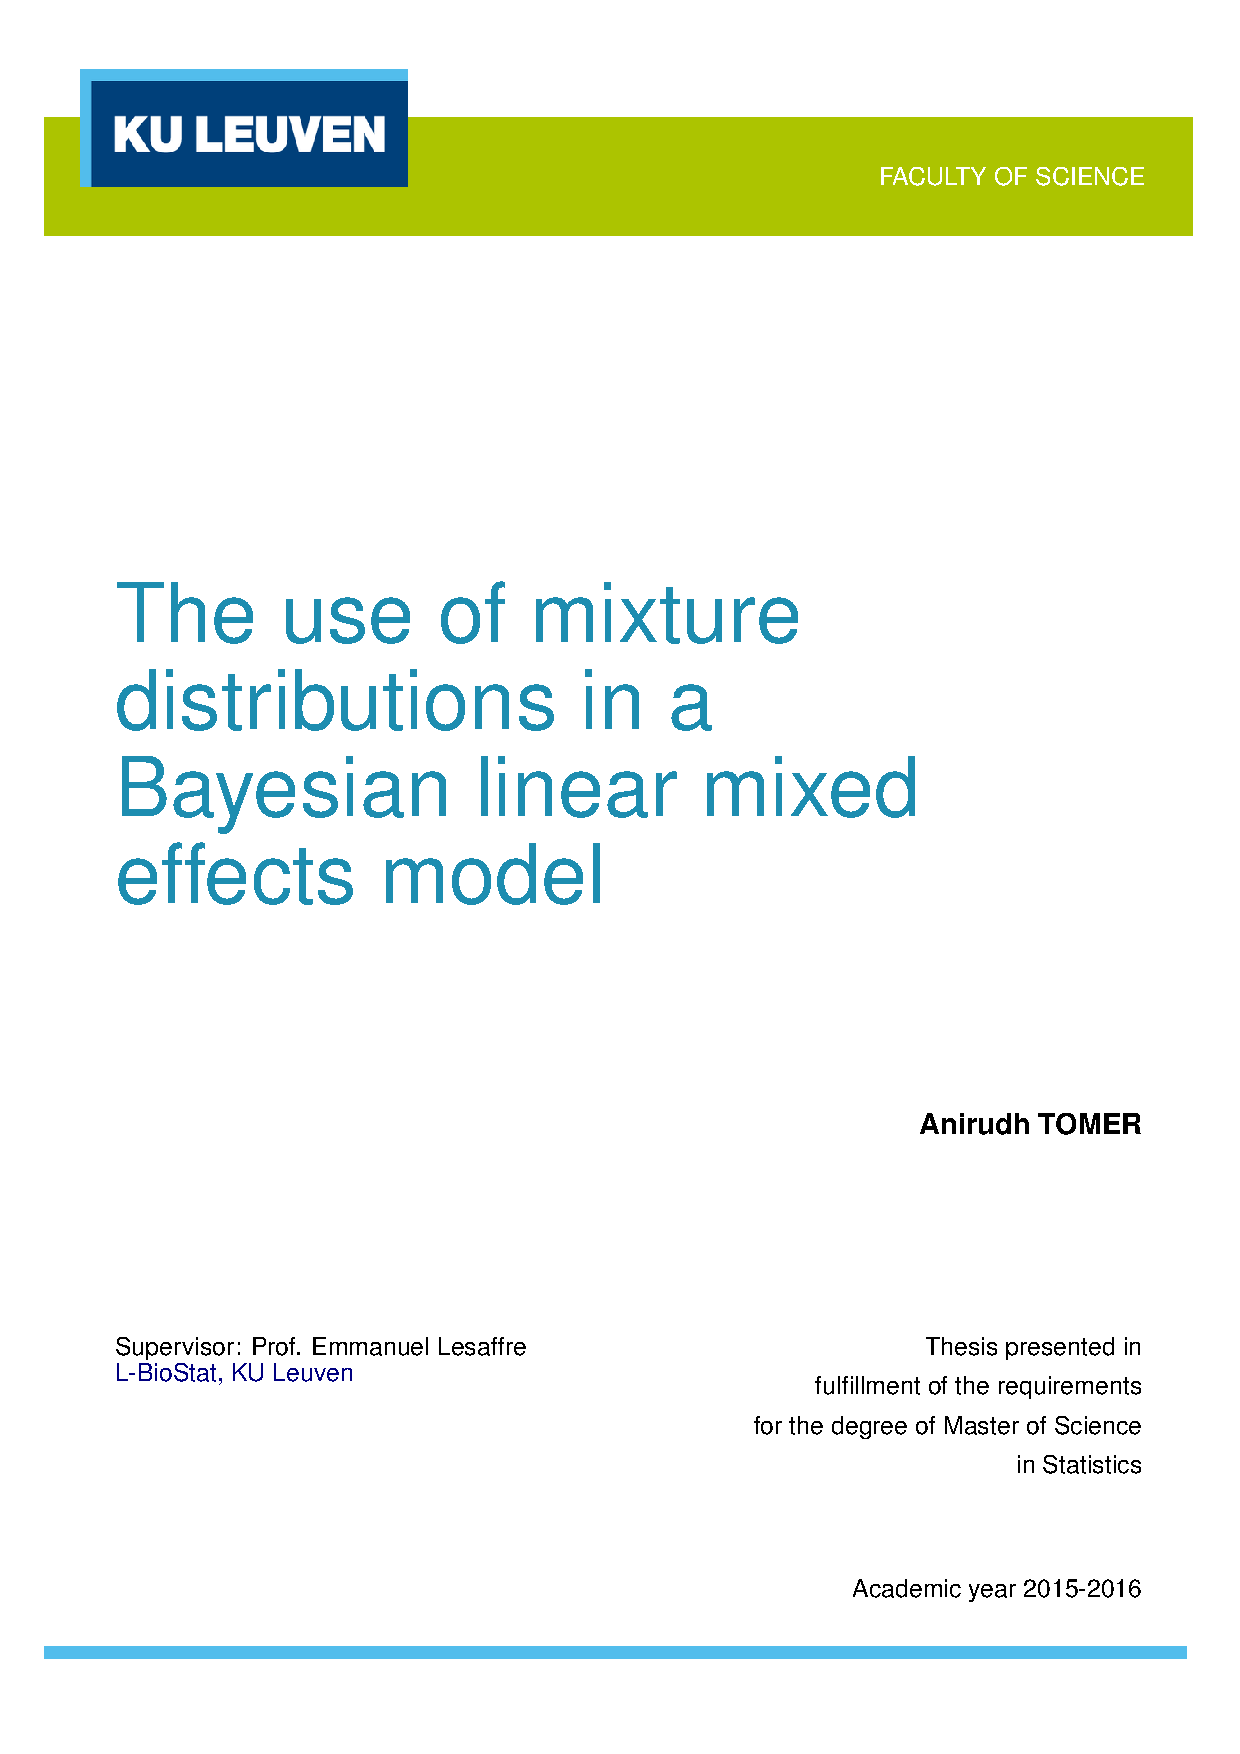
\includepdf[pages={1}]{coverpages/titlepage/titlepage.pdf}
\clearpage \null \clearpage
\null
\vfill
\copyright~ Copyright by KU Leuven \\

Without written permission of the promotors and the authors it is forbidden to reproduce or adapt in any form or by any means any part of this publication. Requests for obtaining the right to reproduce or utilize parts of this publication should be addressed to KU Leuven, Faculteit Wetenschappen, Geel Huis, Kasteelpark Arenberg 11 bus 2100, 3001 Leuven (Heverlee), Telephone +32 16 32 14 01. \\

A written permission of the promotor is also required to use the methods, products, schematics and programs described in this work for industrial or commercial use, and for submitting this publication in scientific contests.
\cleardoublepage

% frontmatter + roman page numbers
\frontmatter

%%%%\include{Chapters/Preface/Preface}\cleardoublepage
%%%%\include{Chapters/Summary/Summary}
%\printglossary[type=\acronymtype,style=list,title={List of abbreviations}]
\cleardoublepage
\tableofcontents

% main matter (chapters + appendices
\mainmatter


% Appendices should go here
\appendix
\chapter{Essential code}

% backmater => mainly references
\backmatter
\printbibliography
\cleardoublepage


\includepdf[pages={1}]{coverpages/backpage/backpage.pdf}
\end{document}
